\documentclass{article}

\usepackage[margin=2.5cm]{geometry}
\usepackage{amsmath,amssymb}
\usepackage{float}
\usepackage{graphicx}
\usepackage{fancyhdr}
\pagestyle{fancy}
\usepackage{tcolorbox,listings}
\usepackage{color}
\usepackage{hyperref}
\renewcommand\headrulewidth{1pt}
\usepackage{marvosym}
\usepackage{xcolor}
\usepackage{tikz}
\usepackage{babel}
\usepackage[french]{babel}
\usepackage[babel=true,kerning=true]{microtype}
\usepackage{afterpage}
\usepackage{wrapfig}
% \usepackage[colorlinks=true,urlcolor=blue]{hyperref}

\newcommand\myemptypage{
    \null
    \thispagestyle{empty}
    \addtocounter{page}{-1}
    \newpage
}

\usetikzlibrary{
    arrows,
    calc,
    shapes.geometric,
    shapes.misc,
    shapes.symbols,
    shapes.arrows,
    automata,
    through,
    positioning,
    scopes,
    decorations.shapes,
    decorations.text,
    decorations.pathmorphing,
    shadows}

\definecolor{darkWhite}{rgb}{0.94,0.94,0.94}

\lstset{
    backgroundcolor=\color{darkWhite},
    breakatwhitespace=false,
    breaklines=true,
    captionpos=b,
    commentstyle=\color{green},
    deletekeywords={...},
    escapeinside={\%*}{*)},
    extendedchars=true,
    keepspaces=true,
    keywordstyle=\color{blue},
    %language=Python,
    morekeywords={*,...},
    showspaces=false,
    showstringspaces=false,
    showtabs=false,
    stepnumber=1,
    stringstyle=\color{gray},
    tabsize=4,
}

\lstdefinestyle{frameStyle}{
    basicstyle=\sffamily,
    numbers=left,
    numbersep=20pt,
    numberstyle=\tiny\color{black}
}

\tcbuselibrary{listings,skins,breakable}

\newtcblisting{customFrame}{
    arc=0mm,
    top=0mm,
    bottom=0mm,
    left=3mm,
    right=0mm,
    width=\textwidth,
    listing only,
    listing options={style=frameStyle},
    breakable
}

\fancyhead[L]{ALLEMAND Fabien\\BALAKRISHNAN Sylvain\\BONNAIL Julie}
\fancyhead[C]{Mesurer les Infrastructures Routières}
\fancyhead[R]{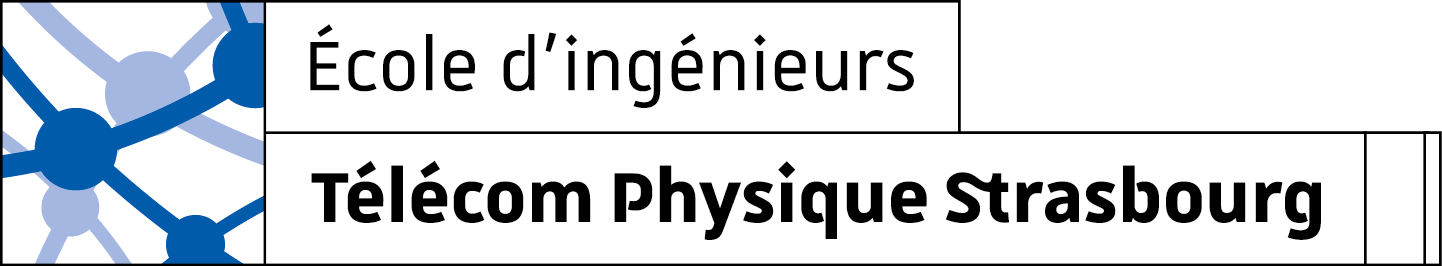
\includegraphics[scale=0.4]{../../common/logo_TPS_1.png}}
\fancyfoot[L]{Projet Ingénieur}
\fancyfoot[R]{\today}

\begin{document}

\thispagestyle{empty}
\addtocounter{page}{-1}
\begin{center}
    \baselineskip=50pt
    \vspace*{1cm}
    \textbf{{\Huge Projet Ingénieur}}\\
    \vspace*{0.25cm}
    \textbf{{\Huge Mesurer les Infrastructures Routières}}\\
    \vspace*{0.25cm}
    \begin{minipage}[c]{.46\linewidth}
        \centering
        \textbf{Equipe:}\\
        ALLEMAND Fabien\\BALAKRISHNAN Sylvain\\BONNAIL Julie
    \end{minipage}
\end{center}
\vspace*{0.1cm}

\begin{figure}[H]
    \centering
    \centerline{
\includegraphics[scale=.66]{../../common/logo_Alcatel_1.png}}
    \vspace*{0.1cm}
    \centerline{
\includegraphics[scale=1.25]{../../common/logo_TPS_2.png}}
\end{figure}

\newpage
\renewcommand{\contentsname}{Table des matières}
\tableofcontents

\newpage
\addcontentsline{toc}{section}{Liste des figures}
\renewcommand{\listfigurename}{Liste des figures}
\listoffigures

\newpage
\vspace*{0.01cm}

\section{Introduction}
Road infrastructures are key when it comes to traveling. Whether it is for daily commuting or one-time journeys, millions of people drive their vehicle on the road in order to go from a point A to a point B.\\
There is no denying that the state of deterioration of roads has a huge impact on the security of the drivers and passengers. An unexpected hole on a road can lead a conductor to change direction abruptly or loose control of the vehicle.\\
The effect of a poorly maintained road on vehicle is usualy overlooked but it seems logical that holes and bumps on a road are likely to cause damage on cars reducing security and increasing maintenance costs on the vehicle.\\
At a larger scale, transportations can be slown down by deteriorated roads meaning the entiere process of economical exchanges is running at a slower pace, hurting the economy of cities or even countries.\\
Finally, the military force of a country can be evaluated by the state of roads networks. In case of emergency, military forces need to move quickly. Once again, the state of the roads is a key factor.\\

The goal of this project is to develop an AI-based solution in order to facilitate road maintenance. By training an AI to recognize degradation on a road, road wrokers could more easily service roads and thus improve security and user experience.\\
In this study, the AI will be mostly trained on acceleration data measured on vehicles. In order to work properly, the model must be able to detect various degradations (bumps and obstacles, holes and cracks as well as gravel) independently of the type of vehicle the data is coming from.\\
For the purpose of the study, two methods will be used in order to collect acceleration data. First, using an Arduino and an IMU. In a second time, by using smartphones accelerometers.
% Different approaches can be used in order to collect acceleration data. The easiest is to create a simple device with an IMU that records data localy requiring human interaction in order to transfer data. Another way to access such type of data is to use accelerometers located in smartphones...
\\
As a proof of concept, a smartphone application will be created and will demonstrate the effectiveness of this road quality assessment method.\\

\section{Rappels R1 et R2}
Comme pour tout projet, les premières étapes avaient consisté à comprendre la problématique, les enjeux et les défis.
Nous avions effectué quelques recherches sur l'évaluation de la qualité des routes et sur des sujets connexes afin de connaître les solutions existantes ou les méthodes pertinentes.

Nous avions ensuite pu définir les objectifs des sprints et les organiser en utilisant les \textit{user stories} et la complexité des sprints. Les sprints avaient ensuite été utilisés pour planifier l'avancement du projet.

Le projet avait été divisé en trois parties:
\begin{itemize}
    \item Collecter des données
    \item Construire et entraîner une intelligence artificielle
    \item Développer une application Android
\end{itemize}

Grâce au petit dispositif à base d'Arduino, nous avions pu réaliser de premiers enregistrements, commencer à analyser ces données et les comparer aux données provenant des deux autres sources que nous avons à disposition (les données de M. Helbert et les données du jeu de données trouvé sur internet).

\begin{figure}
    \center
    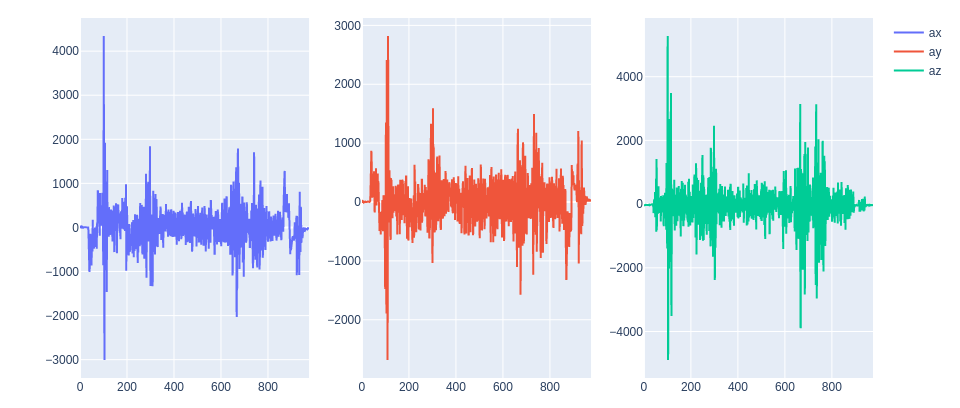
\includegraphics[scale=0.5]{img/DATA9.png}
    \caption{Données accélérométriques enregistrées sur le robot Scout 2.0 avec le dispositif Arduino}
    \label{bump_1}
\end{figure}

% \noindent
% \begin{minipage}[!hc]{0.12\textwidth}
%    \textbf{Remark}
% \end{minipage}
% \vrule\enskip\vrule\quad\begin{minipage}{\dimexpr 0.87\textwidth-0.8pt-1.5em}
% The sampling frequency (i.e. horizontal granularity) is defined by the Arduino program as: \(f = \frac{1}{10 \times 10^{-3}}\) which correspond to a delay of 10 ms between two measures.\\
% It is important to pay attention to the vertical scale of each graph.
% \end{minipage}

En parallèle, nous avions aussi débuté le développement d'une application Android pour permettre d'enregistrer des données plus précises et de façon plus efficace.

\section{Application Android}


\section{Collecte de Données}
\label{data_collection}

Dans notre projet de détection de détériorations de la route, la collecte de données est une étape fondamentale pour garantir la qualité et la fiabilité de notre modèle. Nous avons donc réalisé une nouvelle collecte de données en utilisant le robot, le module Arduino et notre application de collecte de données. Cette fois-ci, notre objectif était de collecter un maximum de données de différents types de détériorations de la route, afin d'en avoir suffisamment pour entraîner notre modèle d'apprentissage automatique.

Nous avons collecté environ quatre-vingt données (Figure \ref{data_collection_1}) de différentes détériorations de la route, notamment des dos d'âne, des failles, des fissures et des affaissements. Pour chaque type de détérioration, nous avons collecté en moyenne dix données par dégradation pour garantir la diversité de nos données.

Cependant, nous avons rencontré un problème avec notre carte arduino lors de la collecte de données. En effet, celle-ci n'a enregistré qu'une dizaine de données, sans que nous puissions identifier la cause de cette erreur. Bien que ce soit une déception, nous avons malgré tout pu collecter suffisamment de données avec l'application Android pour poursuivre notre projet de détection de détériorations de la route.

Dans l'ensemble, la collecte de données est une étape cruciale de notre projet, car la qualité des données collectées aura un impact direct sur la qualité et l'efficacité de notre modèle.

\begin{figure}
    \center
    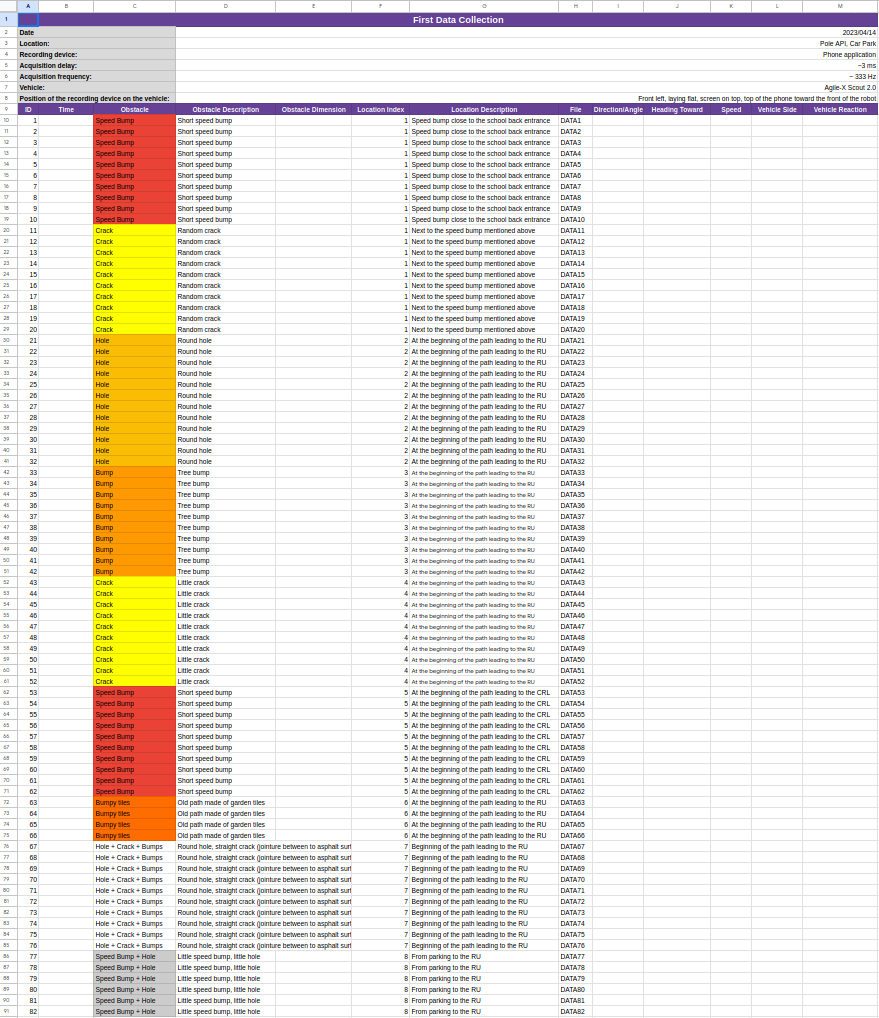
\includegraphics[scale=0.5]{img/data_collection_1.png}
    \caption{Tableur récapitulatif de la collecte de données}
    \label{data_collection_1}
\end{figure}

\section{Augmentation des Données}
Le jeu de données obtenu suite à la séance d'enregistrement décrite dans la Section \ref{data_collection} est constitué de quatre-vingt-deux enregistrements résumés dans la Table \ref{data_collection_table}. Tel quel, ce jeu de données est insuffisant pour procéder directement à l'entraînement d'un modèle d'intelligence artificielle. En effet, pour entraîner les modèles les plus simples, il faut être en possession de suffisamment de données pour créer des jeux d'entraînement, de validation et de test. Les méthodes plus avancée relevant de l'apprentissage profond nécessitent encore plus de données d'entraînement pour être utilisées dans de bonnes conditions et offrir des résultats corrects.

Plutôt que de continuer à collecter des données, une démarche longue et peu instructive, nous avons choisi de procéder à de l'augmentation de données.

Les méthodes de \textit{data augmentation} consistent à créer de nouvelles données en altérant légèrement les données déjà présentes dans le \textit{dataset}. Lorsqu'on travaille sur des images, de nouvelles images peuvent être créer en effectuant des rotations, en rognant l'image ou en modifiant certaines propriétés (contraste, luminosité...).\\
Dans le cadre de ce projet, les données sont sous la forme de séquences numériques selon trois axes. Nous avons choisi cinq méthodes pour augmenter la quantité de données:
\begin{itemize}
    \item Renverser la séquence dans le temps
    \item Inverser l'axe correspondant à la rotation du robot
    \item Ajout de bruit
    \item Ajout d'un signal porteur
    \item Découpage des séquences
\end{itemize}

\begin{table}[]
    \begin{tabular}{|l|c|}
    \hline
    Dégradation  & \multicolumn{1}{l|}{Nombre d'enregistrements} \\ \hline
    Ralentisseur & 20                                            \\ \hline
    Racines      & 10                                            \\ \hline
    Fissure      & 20                                            \\ \hline
    Trou         & 12                                            \\ \hline
    Dalles       & 4                                             \\ \hline
    Parcours     & 16                                            \\ \hline
    \end{tabular}
    \caption{Table résumant la collecte de données}
    \label{data_collection_table}
\end{table}

\subsection{Renverser la séquence dans le Temps}
Etant donnée que le robot est très réactif (l'accélération et la décélération sont similaires), nous pouvons considérer que la séquence renversée dans le temps reste représentative. (Figure \ref{data_augmentation_1})

\begin{figure}
    \center
    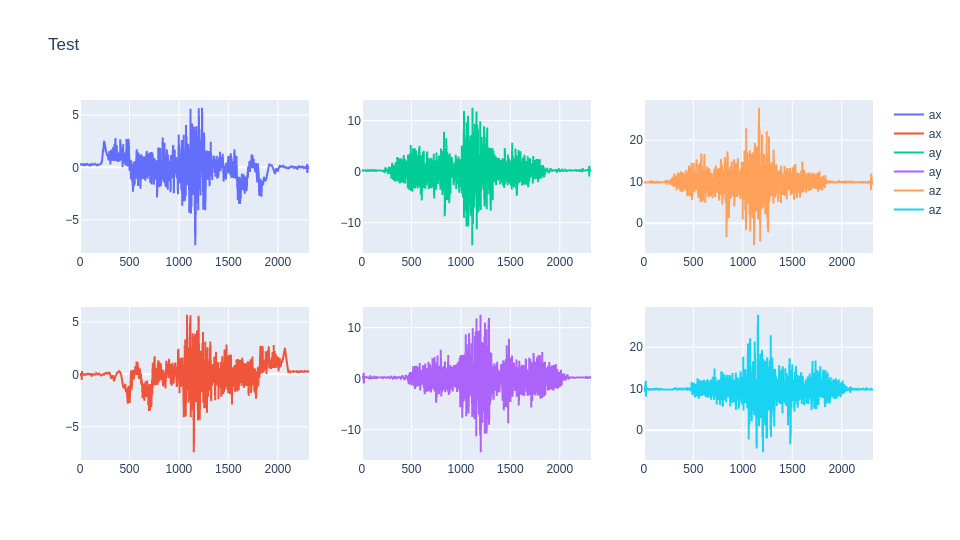
\includegraphics[scale=0.5]{img/reversed_data.png}
    \caption{Comparaison de enregistrement et de sa version modifiée (renversement du temps)}
    \label{data_augmentation_1}
\end{figure}

\subsection{Renverser l'Axe de Rotation}
De la même façon, inverser la rotation du robot ne modifie pas l'enregistrement du point de vue des dégradations de la route. Les dégradations ont principalement un effet sur l'axe vertical et n'impactent pas la direction du robot donc nous pouvons prendre l'opposée des valeurs sur l'axe X. (Figure \ref{data_augmentation_2})

\begin{figure}
    \center
    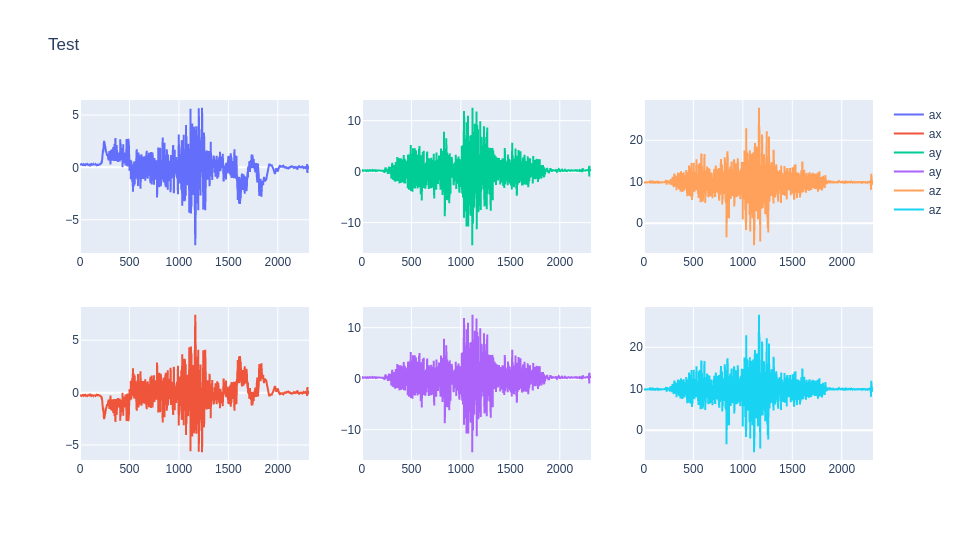
\includegraphics[scale=0.5]{img/inverted_data.png}
    \caption{Comparaison de enregistrement et de sa version modifiée (renversement d'un axe horizontal)}
    \label{data_augmentation_2}
\end{figure}

\subsection{Ajout de Bruit}
Une méthode classique pour augmenter la quantité de données consiste à ajouter du bruit. Cette méthode s'applique dans une certaine mesure aux données accélérométriques recueillies. Un faible bruit peut simuler un bitume moins lisse mais un trop gros bruit signifierait que la route est dans un mauvais état global (gravier...). (Figure \ref{data_augmentation_3})

\begin{figure}
    \center
    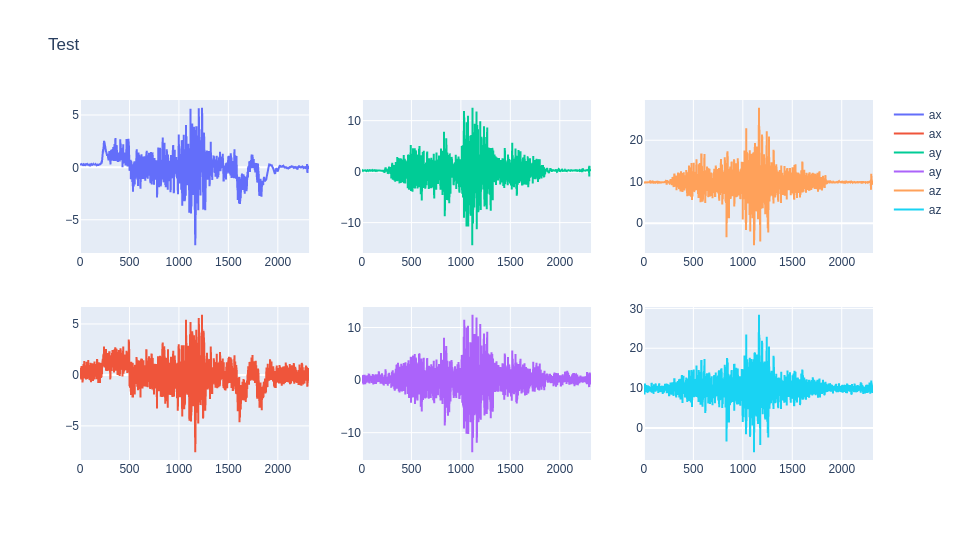
\includegraphics[scale=0.5]{img/noisy_data.png}
    \caption{Comparaison de enregistrement et de sa version modifiée (ajout de bruit)}
    \label{data_augmentation_3}
\end{figure}

\subsection{Ajout d'un Signal Porteur}
Des recherches sur internet \cite{TerryUm_ICMI2017} nous ont montré qu'il est aussi possible d'ajouter un signal porteur pour simuler un dénivelé supplémentaire. Un enregistrement de passage dans trou sur un sol horizontal peut devenir un enregistrement de passage dans un trou au cours d'une montée.

\subsection{Découpage des Séquences}
Une dernière méthode simple de \textit{data augmentation} consiste à découper les séquences dans le temps pour isoler les dégradations lors de parcours ou tout simplement pour obtenir des séquences de longueur différentes avec le passage sur la dégradation à différents moments de l'enregistrement (pas nécessaireemnt au milieu) ce qui pourrait induire un biais d'apprentissage.

Finalement, les méthodes précédentes peuvent être combinées afin de générer de nouvelles séquences artificielles.

\section{Intelligence Artificielle}
Ayant suffisemment de données pour entraîner un modèle d'intelligence artificelle, nous avons commencé à mettre les données en forme pour faciliter l'apprentissage.

\subsection{Création du Jeu de Données}
La première étape consiste à créer un véritable jeu de données labélisé en utilisant les enregistrements et les labels recuillis lors des collectes de données.
Pour cela nous avons suivi dans le grandes lignes un tutoriel de pré-traitement des données séquentielles pour classification.\cite{tuto_1} Nous avons donc créé un grand \textit{dataset} contenant les \textit{inputs} regroupant tous les enregistrements que nous avons stocké sous la forme d'un fichier \textit{csv} et un fichier de lables avec l'extension \textit{.labels} qui regroupe les fichiers et leurs labels.

\subsection{Premiers Modèle}
La mise en place d'un premier modèle en suivant un autre tutoriel s'est avérée infructueuse. Adapter le programme présenté dans le tutoriel ne permettait pas d'utiliser le modèle car il nécessite des séquences de longueurs égales, ce qu in'est pas le cas dans nos données.\cite{tuto_2} Il faut donc ajouter une étape suplémentaires de pré-traitement pour obtenir des séquences de même longueur (par découpage ou ajout de \textit{padding}).

\subsection{Méthodes Envisagées}
Au cours des prochains sprints, nous envisageons de poursuivre le développement de l'intelligence artificielle.

Nous commencerons par des modèles simples comme le modèle \textit{k-Nearest Neighbors} rencontré à plusieurs reprises lors de nos recherches. Nous pensons aussi essayer des méthodes plus avancées basées sur des approches d'apprentissage profond comme par exemple les \textit{Long-Short Term Memory} (LSTM) qui sont très utilisés pour la classification de séquences numériques. Finalement, nous essairons d'entraîner un modèle de détection d'anomalies. Bien qu'il n'effectue pas une classification des anomalies, ce modèle a l'avantage de détecter tout type d'anomalie et serait donc capable d'identifier n'importe quel type de dégradation de la chaussée.

Suivant les ressources qui seront à notre disposition, nous devrons éventuellement effectuer l'entraînement des approches \textit{deep learning} par affinement d'un modèle déjà existant pour une tâche simialire (comme la détection de chute) voire plus générale et nous espérons pouvoir mettre en place un programme capable d'effectuer un apprentissage continu grâce à de nouvelles données enregistrées au fur et à mesure.

\section{Conclusion}
Having understood the subject, its issues and constraints, having created supports to use the sensors and having started to collect our first accelerometric data, we can move on to the next stage of the project. Between now and the next review, we plan to analyze the data collected. This will give us an idea of the artificial intelligence model to use. Once this is done, we will have to collect more data so that the selected models are trainable and as accurate as possible. We will then be able to compare the models and choose which one(s) we will select for the rest of the project. Finally, we will also start to develop the mobile application because it can be done in parallel with the artificial intelligence part.

\newpage
\vspace*{0.01cm}
\addcontentsline{toc}{section}{Bibliographie}
\renewcommand{\refname}{Bibliographie}
\bibliographystyle{plain}
\bibliography{bibliography.bib}

\end{document}